% !TEX root = ../notes.tex

% ================  Unsupervised Learning ==============

\section{Unsupervised Learning}

In this section we will look at how machines can learn from data without human intervention as opposed to \emph{Supervised Learning}. The goal of Unsupervised Learning is to go from our dataset $X$ to a function $f(X)$, a simpler representation of the data. We can already categorize Unsupervised Learning in two categories :
\begin{itemize}
	\item Clustering for discrete data.
	\item Matrix factorization, Kalman filtering, unsupervised neural networks, etc... for continuous data.
\end{itemize}

\subsection{Clustering in general}

Going from a set of points with a distance metric between points to \textbf{groups} into some clusters. The goal is to perform same labelling for members that are close/similar to each other (Closeness can take on many shapes as we will see later), therefore members belonging to different clusters should be dissimilar. 

The main use cases of clustering is having points in a high-dimensional space. Similarity/Distance is defined using some distance measures such as Euclidian, Cosine, Jaccard, edit distance, etc. The choice of such metrics is determinant regarding the performance and accuracy of the clustering, it is consequently a huge advantage to have a domain expert/specialist in order to choose the better metric.

\begin{figure}[H]%---------------FIG--------------
 \centering
 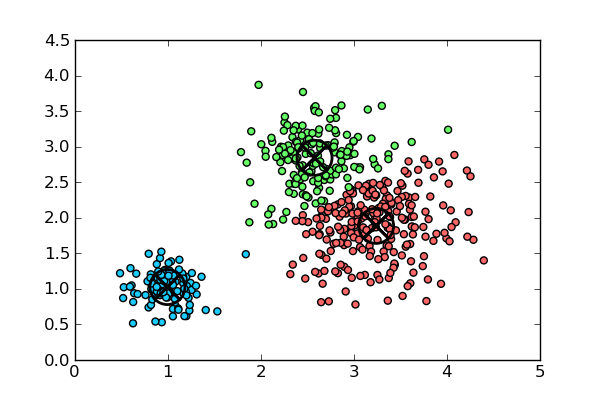
\includegraphics[width=13cm]{./img/09/clustering}
 \caption{\label{pic:clustering} Example of clustering. (K-mean)}
\end{figure}

\subsubsection{Terminology}
There are several way to organize/apply clustering :
\begin{itemize}
  \item \textbf{Point assignment}: Maintains a set of clusters. The points belong to ``nearest'' cluster.
  \begin{itemize}
   \item \textbf{Hard clustering}: Every item is uniquely assigned to a cluster.
   \item \textbf{Soft clustering}: Cluster membership is a real valued function, distributed across several clusters. This type of clustering is very agile and useful in many cases.
  \end{itemize}
  \item \textbf{Hierarchical clustering}: Cluster coming from some sort of a hierarchy
  \begin{itemize}
   \item \textbf{Agglomerative} (Bottom-Up): Initially, each point is a cluster. Then, we repeatedly combine the two ``nearest'' clusters into one.
   \item \textbf{Divisive} (Top-Down): We start with only one cluster and recursively split it.
   \item \textbf{Flat clustering: } As opposed to hierarchical clustering, there is no inter-cluster structure.
  \end{itemize} 
\end{itemize}

\subsubsection{Characteristics of Clustering Methods}

In order to better understanding clustering and when/how it should be applied, we have to take a peek at the characteristics of Clustering methods, namely :
\begin{itemize}
	\item \textbf{Quantitative} : scalability (how many samples), dimensionality (how many features).
	\item \textbf{Qualitative} : Type of attributes (numerical, categorical, etc.), type of shapes (spheres, hyperplanes, etc.).
	\item \textbf{Robustness} : sensitivity to noise and outliers, sensitivity to the processing order.
	\item \textbf{User interaction} : incorporation of user constraints(e.g., number of clusters, max size of clusters), interpretability and usability i.e. how transparent is the model/ clusterization, black/white boxing c.f. trees/supervised learning.
\end{itemize}

These characteristics influence a great deal over clustering, and even by having them well defined clustering tasks are often found hard in easy looking situations.

\begin{figure}[H] %----------- SubGraph ---------------------
\centerline{
\subfigure{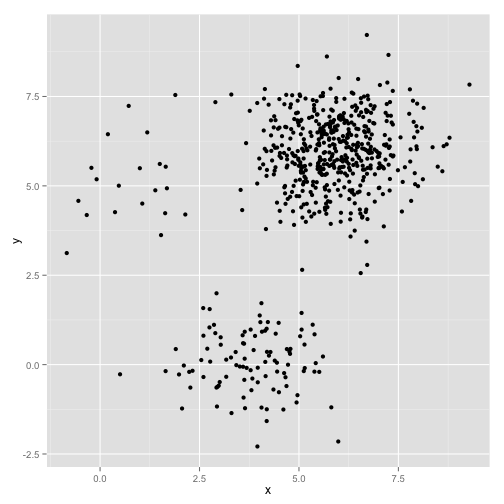
\includegraphics[height=5.5cm]{img/09/cluster_outliers_01}}
\subfigure{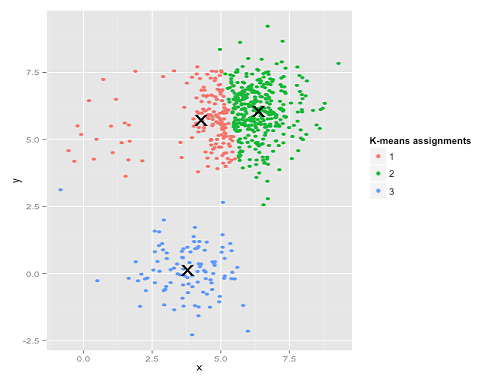
\includegraphics[height=5.5cm]{img/09/cluster_outliers_02}} 
}
\caption{\label{pic:clustering_outliers} 
Image on the left is the raw data. We can see the three different clusters. The image on the left is the result of the K-means showing that outliers can be a problem for clustering the data.
}
\end{figure}

Figure \ref{pic:clustering_outliers} shows what can happen with outliers and a simple clustering algorithm. Indeed, we see that on the left, the three clusters are quite visible. But the K-means algorithm fails to find the three clusters. A very interesting discussion on the drawbacks on K-means can be found on \href{http://stats.stackexchange.com/questions/133656/how-to-understand-the-drawbacks-of-k-means}{StackExchange}.

\subsubsection{Examples of Clustering}

\paragraph{Stereotypical Clustering}
In high dimensionality clustering what may seem to be a right choice in high dimensionality may get bad when projected in 2D, where outliers often appear. Usually to obtain a good clusterisation, we have to accept that some points may not be classified well or even not classified at all because ultimately, the model and it's programmer cannot understand the process that generated the data. Figure \ref{pic:clustering} shows what is a typical stereotypical clustering. 

\paragraph{Clustering for Segmentation}
In the case of an image, it can be usef to segment/cut the image into multiple parts. For example, we would like to get the front, middle and background of an image. An example with K-means is given in Figure \ref{pic:segmentation}.

\begin{figure}[H]%---------------FIG--------------
 \centering
 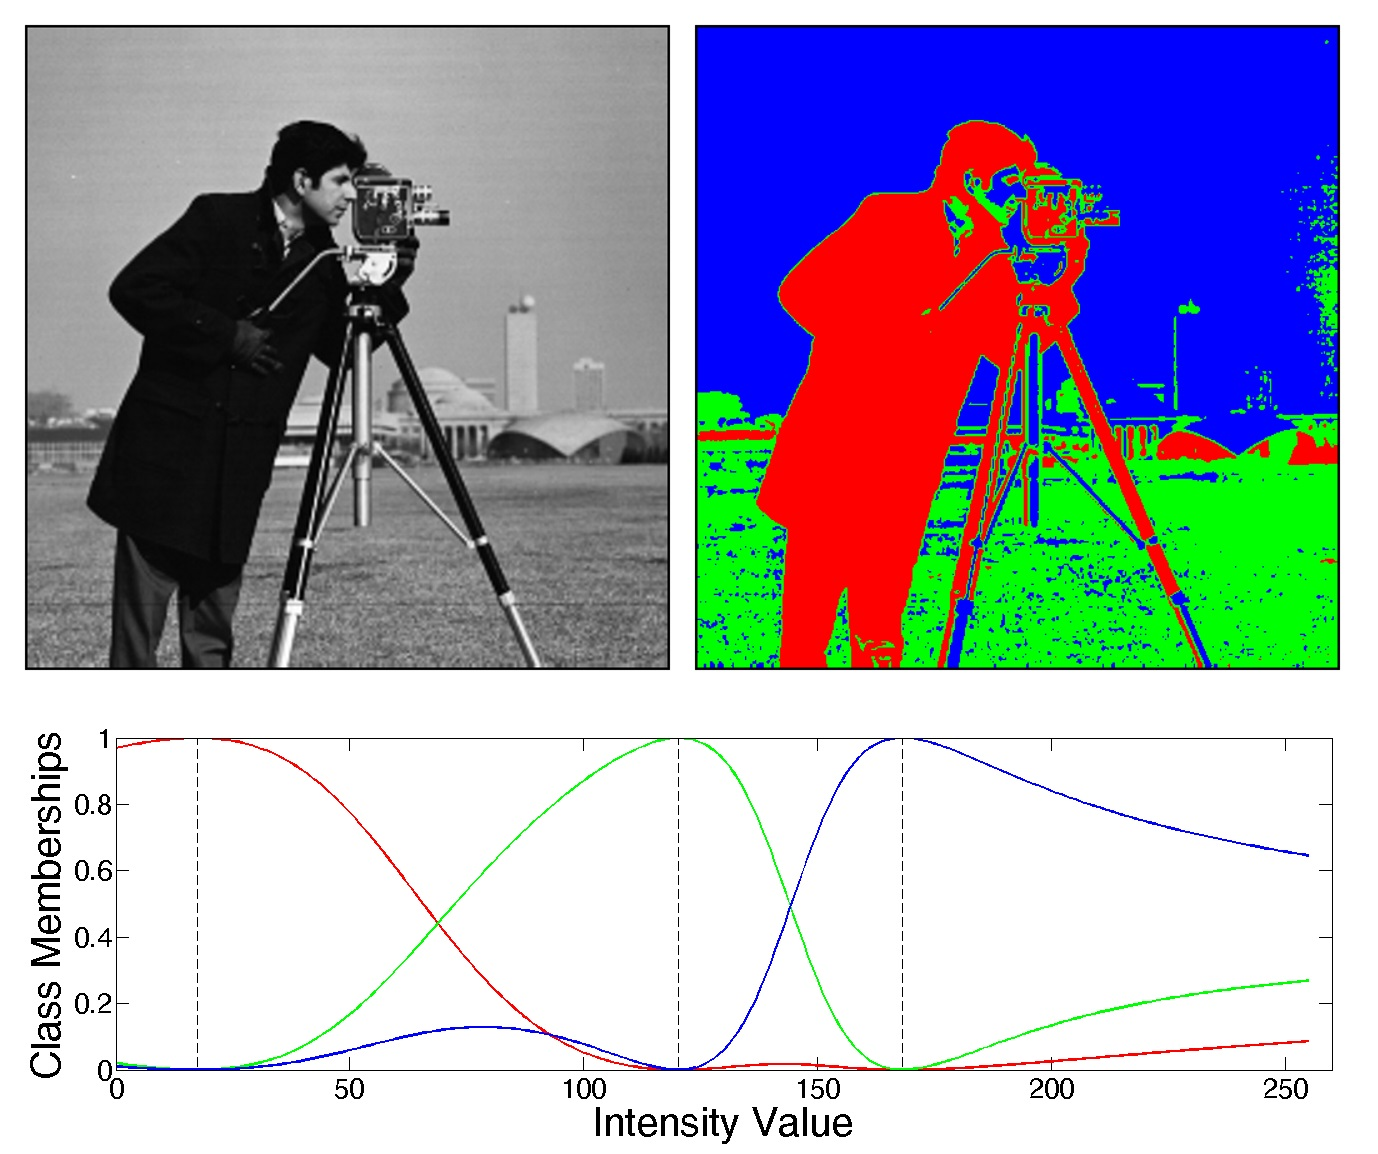
\includegraphics[width=13cm]{./img/09/segmentation}
 \caption{\label{pic:segmentation} Example of segmentation on a black-and-white image. The algorithms used are K-means and Fuzzy C-means (or soft K-means).}
\end{figure}

\paragraph{Condensation/Compression} 

In Figure \ref{pic:compression}, we can infer several models/distributions that are contained into the data. But for a computer it is more difficult to see these underlying regression. Therefore we can use Condensation/Compression to solve this problem. Condensation/Compression doesn't aim to cluster/model the underlying structure, but try to identify and subtract "submodels" in order to yield a simplification, a reduced variance "sample" of the data.

\begin{figure}[H]%---------------FIG--------------
 \centering
 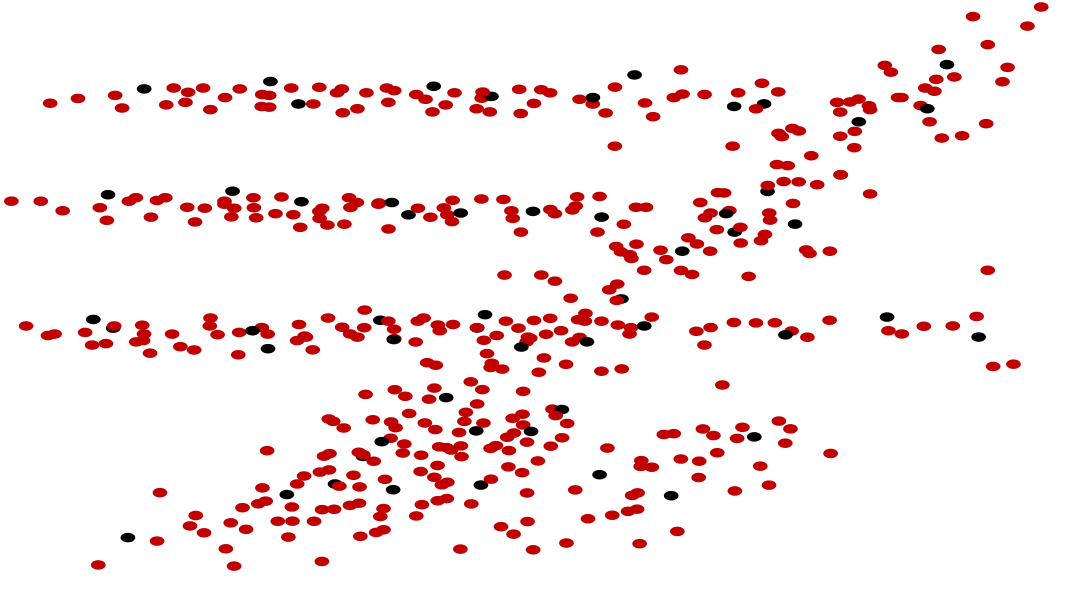
\includegraphics[width=10cm]{./img/09/compression}
 \caption{\label{pic:compression} Example of data that can be compressed using clustering methods.}
\end{figure}

\paragraph{Read more}

The \href{https://en.wikipedia.org/wiki/Cluster\_analysis}{Wikipedia page for clustering analysis} gives different algorithms for clustering and explain different evaluation methods. 

\subsubsection{Cluster Bias}

What is called Cluster Bias or Cluster hallucination comes from the human way of conceptualizing and categorize the world into categories (\emph{exemplars}); we often tend to see cluster structures where there is not really. One of the most common example is the constellations. Nowadays, unsupervised learning is rather cheap. Thus, combined with cluster bias, instances of overuse or unjustified use of clustering are often encountered. A good data scientist has to ask himself if he has meaningful reasons to use clustering. People often assume that domain has discrete classes in it (ex. types of people). In reality the data is usually continuous. 

\subsection{Clustering : A hard problem!}

Here our eternal curse of dimensionality strikes again. The data scientist is often tricked by how clustering looks easy when there are only two dimensions or when there is a small amount of data and it is in most cases true. Nevertheless most applications involve tremendously more than two dimensions and hight dimension spaces look very different from 2D spaces. For example, all points in high dimensions are about the same distance from each other. 

\subsubsection{Read more on this topic}

Three articles on \href{http://alexhwilliams.info/itsneuronalblog/}{Alex Williams' blog}, PhD student in Computational/Theoretical Neuroscience at Stanford University, are talking about clustering in different ways: \href{http://alexhwilliams.info/itsneuronalblog/2015/09/11/clustering1/}{What is clustering and why is it hard?}, \href{http://alexhwilliams.info/itsneuronalblog/2015/10/01/clustering2/}{Is clustering mathematically impossible?}, and \href{http://alexhwilliams.info/itsneuronalblog/2015/11/18/clustering-is-easy/}{Clustering is hard, except when it's not}. These are really interesting articles on different aspects of clustering. They are easy to understand, even the second with its mathematical approach of the clusters.

\paragraph{Music CDs}

We can intuitively divide Music into categories. And we know that some customers will prefer a few categories. But {\bf what are categories really}? We can for example represent a CD by a set of customer who bought it. Then similar (define similar) CDs will have a similar set of customers.

We see in this case that the representation is easy. But the dimensionality explodes quickly, {\it e.g.} Amazon. Therefore, choosing the right encoding is one of the determinant factor.

\paragraph{Documents}

Encoding has a big impact on clustering, in this case the way we define a document as sets of words has a direct impact on the distance metric :
\begin{itemize}
	\item Sets as vectors : cosine distance
	\item Sets as sets : Jaccard distance
	\item Sets as points Euclidian distance
\end{itemize}

\subsection{Hierarchical Clustering}

The key operation of hierarchical clustering is how to repeatedly combine two nearest clusters. There are also several other questions that also arise when speaking about hierarchical clustering such as :
\begin{description}
	\item [How is a cluster of more than one point represented ?]
The key problem is how the "location" of each cluster represented throughout the merging process in order to choose which pair of cluster is closest. In the \textbf{Euclidean case}, each cluster has a \emph{centroid} computed from the average of its data points, note that a centroid doesn't have to be a data point it can be totally artificial. We can also use a \emph{clustroid}, namely the existing data point "closest" to all of the other points according to the following metrics :
\begin{itemize}
	\item Smallest maximum distance to other points.
	\item Smallest average distance to other points.
	\item Smallest sum of squares of distances to other points.
\end{itemize}
	\item [How is the "nearness" metric of cluster determined ?]
We can measure the nearness between clusters according to different approaches:
\begin{enumerate}
	\item \emph{Intercluster distance} : Minimum of the distances between any two points, one from each cluster.
	\item \emph{Cohesion} : Pick a metric e.g. maximum distance from the clustroid for example. And then merge clusters whose union is most cohesive. Cohesion can also be : \emph{diameter} of the merged cluster (max distance between points in the cluster), \emph{average distance} between points in the cluster, \emph{density-based approach} (ex: for geolocation data) see after.
\end{enumerate} 
	\item [When should we stop combining clusters ?] 
	It is always difficult to decide when we should stop clustering. One way would be to compute some measure of \emph{how well the clustering fits}. For example, we can use a sum of distances from cluster centres. Then, we can check if the graph of the error in function of the number of clusters has an elbow. Finally, we can choose the number of cluster minimizing this measure. Another way to check if the clustering is still good is to use the \href{https://en.wikipedia.org/wiki/Silhouette\_(clustering)}{silhouette} score. 
\end{description}

\begin{figure}[H]%---------------FIG--------------
 \centering
 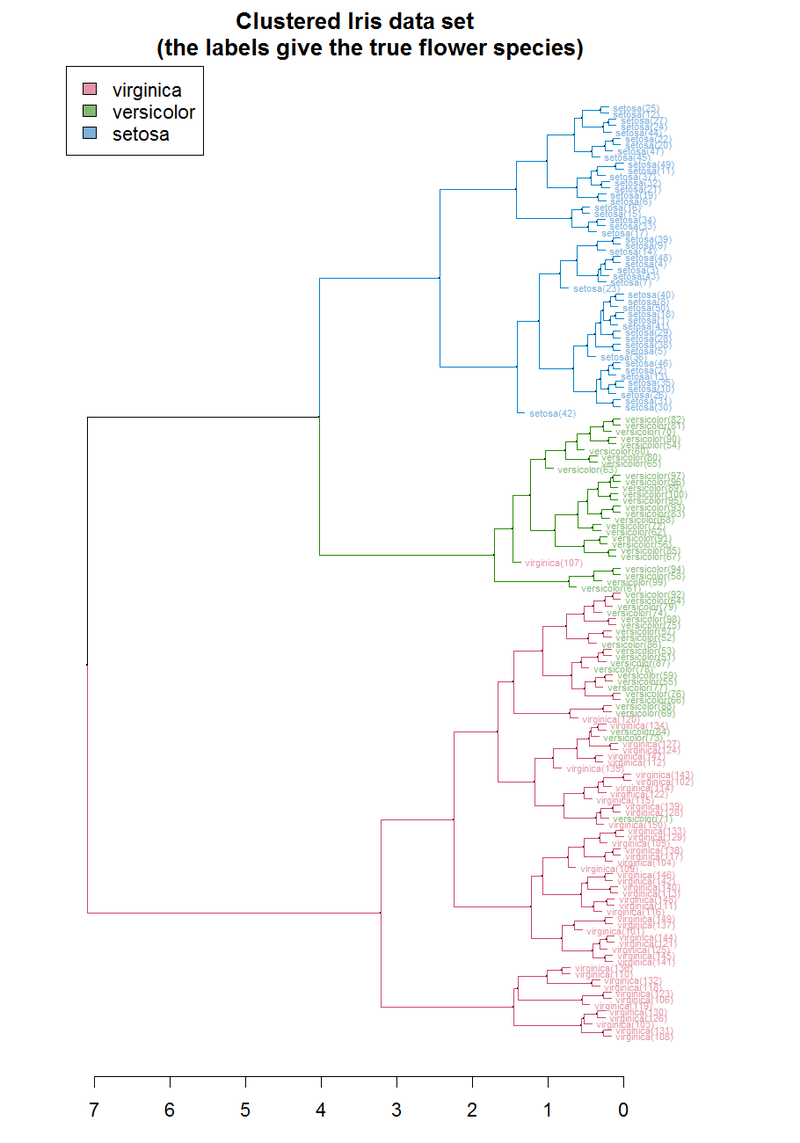
\includegraphics[width=13cm]{./img/09/Iris_dendrogram}
 \caption{\label{pic:dendrogram} Dendogram of the Iris data set. The hierarchical clustering has been done using a {\bf agglomerative} algorithm.}
\end{figure}

\subsubsection{Implementation of hierarchical clustering} 

The naive implementation of the hierarchical clustering can be done using the pairwise distances between all pairs of clusters. But computing this pairwise distance and merging them has a total complexity of $O(N^{3})$. A more clever approach using better indexing structures such as priority queues can improve performance up to a $O(N^{2}\log(N))$ complexity. Nevertheless, it is still too complex for big dataset not fitting into the memory.

\subsection{K-means Clustering}

\subsubsection{Standard K-means}

The standard K-means algorithm is based on \textbf{Euclidean distance}, the quality measure is \textbf{intra cluster} only. It is a simple greedy algorithm that locally optimizes the quality measure. The algorithm resumes to the following two steps :
\begin{itemize}
	\item \textbf{Finding the closest cluster center} for each item and assign it to that cluster.
	\item \textbf{Recompute the cluster centroid} as the mean of the items, having added the new item to the cluster.
\end{itemize}
The most challenging and impactful decisions when using K-means is to choose the number of clusters and also to pick the initial cluster centres. The latter can be done by sampling the input data or following more complex methods as described later. We also have to choose when to stop iterating by either :
\begin{itemize}
	\item Defining a fixed number of iterations.
	\item Until no changes in assignments happen.
	\item Until there are only small changes in quality.
\end{itemize}
As we said previously, \textbf{Initialization} is the most crucial part when running K-mean, we can choose to pick a random subset of k points from dataset or use methods like K-Means++ that iteratively constructs a random sample with good spacing across the dataset. However you choose the method for choosing your initial points, take into account the fact that optimal K-Means clustering is a NP-hard problem and that randomization helps avoiding bad configurations and saves up a lot of time/complexity.

\subsubsection{K-means++}
The idea of the K-means++ algorithm is the following:
\begin{description}
 \item[Start] Choose the first cluster center at random from the data points
 \item[Iterate] 
 \begin{itemize}
  \item For every remaining data point $x$, compute $D(x)$ the distance from $x$ to the closest cluster center.
  \item Choose a remaining point $x$ randomly with probability proportional to $D^2(x)$, and make it a new cluster center.
 \end{itemize}
\end{description}

Intuitively, this finds a sample of widely-spaced points avoiding ``collapsing'' of the clustering into a few internal centers.

\subsubsection{K-means properties}

Here are some properties of the K-means algorithm:
\begin{itemize}
 \item It's a greedy algorithm with random setup. Therefore, the {\bf solution is not optimal} and varies significantly with different initial points.
 \item It has a very simple convergence proof.
 \item The {\bf performance is in $O(nk)$ per iteration}, $n$ being the total features in the dataset and $k$ the number of clusters. It is quite good and it cannot be heuristically improved.
 \item There are many generalizations;
 \begin{itemize}
  \item Fixed-size clusters
  \item Simple generalization to m-best soft clustering
 \end{itemize}
 \item As a ``local'' clustering method, it works well for data condensation/compression.
\end{itemize}

\subsubsection{K-means drawbacks}

Every time an algorithm has good properties, it will have drawbacks. Here are some of them:
\begin{itemize}
 \item It often terminates at a {\bf local optimum}.
 \item It needs a {\bf distance function} to compute the mean.
 \item It needs to specify {\bf K} in advance.
 \item It does not handle {\bf noisy data and outliers}.
 \item Clusters {\bf only} have {\bf convex shapes}.
\end{itemize}

\subsubsection{How to choose K?}

In order to choose K, we can use the same techniques as when we have to stop the clustering in the hierarchical clustering. The idea would be:
\begin{itemize}
 \item We execute the clustering for $K=1,2,3,...$
 \item We define $J$ as the ``average within cluster sum of squares''
 \item We plot $J$ against K.
 \item We pick K suchat that $J(K) \simeq J(K+1)$
\end{itemize}
